\section{目标检测方法}

\begin{frame}[allowframebreaks]
    \frametitle{\textsc{目录}} \vspace{-0.3cm}
    \begin{spacing}{0.0}
        \tableofcontents[currentsection,hideallsubsections]
    \end{spacing}   % 若不想要目录, 注释掉该句
\end{frame}

\begin{frame}
    目标检测有两个主要流派:Anchor-based与Anchor-Free,两类算法的主要区别在于算法当中是否有预设锚框\\
    \begin{itemize}
        \item[$ \bullet $] Anchor-based:YOLOv2、SSD、Faster \;R-CNN
        \item[$ \bullet $] Anchor-Free:YOLOv1、CornerNet、CenterNet、FCOS
    \end{itemize}

    \vspace{1em}
    另外一个划分是:一阶段和二阶段算法,阶段主要是指从输入到结果之间网络模型的运算次数\\
    \begin{itemize}
        \item[$ \bullet $] 一阶段:YOLO、SSD、CornerNet、CenterNet、FCOS
        \item[$ \bullet $] 二阶段:R-CNN、Faster \;R-CNN
    \end{itemize}

    \vspace{1em}
    在后面的算法当中将介绍二阶段Anchor-based算法Faster\quad R-CNN和一阶段Anchor-Free算法YOLOv1\\

\end{frame}


\begin{frame}
    \noindent\large\textbf{基础知识}
    \begin{itemize}
        \item[$ \bullet $] 矩形框的3种表示
            矩形框的表示形式有:\\
            $[x,y,w,h]$ \\
            $[x_1,y_1,x_2,y_2]([left,top,right,bottom])$\\
            $[cx,cy,w,h]$
        \item[$ \bullet $] 交并比(IoU)
            交并比是指两个矩形的交集与并集的面积之比$IoU=\frac{|A\cap B|}{|A\cup B|}$,
            实现是采用第二种矩形表示进行实现$A[l_A,t_A,r_A,b_A],B[l_B,t_B,r_B,b_B]$:\\
            $S_A=(r_A-l_A)\times(b_A-t_A)$\\
            $S_B=(r_B-l_B)\times(b_B-t_B)$\\
            $W_{AB}=(min(r_A,r_B)-max(l_A,l_B))$\\
            $H_{AB}=(min(b_A,b_B)-max(t_A,t_B))$\\
            if $ W_{AB}<0$ or $H_{AB}<0$ then $IoU = 0$\\
            else $IoU=\frac{W_{AB}\times H_{AB}}{S_A+S_B-W_{AB}\times H_{AB}}$
            % \hspace{10cm}
            \vspace{-3.5cm}
            \begin{figure}
                \hspace{6cm}
                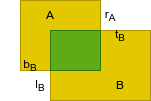
\includegraphics[width=0.4\linewidth]{iou.png}
            \end{figure}
    \end{itemize}
\end{frame}

\begin{frame}
    \large
    \textcolor{vscodedef}{def}  \textcolor{vscodefuncation}{box\_iou}\textcolor{vscodebracket}{(}\textcolor{vscodeparameter}{boxes1}: \textcolor{vscodeclass}{Tensor}, \textcolor{vscodeparameter}{boxes2}: \textcolor{vscodeclass}{Tensor}\textcolor{vscodebracket}{)}->\textcolor{vscodeclass}{Tensor}:\\
    \vspace{0.2em}
    \qquad\textcolor{vscodecomment}{\# boxes1:(N,4) boxes2:(M,4) use 'xyxy'}\\
    \vspace{0.2em}
    \qquad\textcolor{vscodeparameter}{area1}=\textcolor{vscodebracket}{(}\textcolor{vscodeparameter}{boxes1}\textcolor{vscodecomment}{[}:,\textcolor{vscodecomment}{2]}-\textcolor{vscodeparameter}{boxes1}\textcolor{vscodecomment}{[}:,\textcolor{vscodecomment}{0]}\textcolor{vscodebracket}{)}*\textcolor{vscodebracket}{(}\textcolor{vscodeparameter}{boxes1}\textcolor{vscodecomment}{[}:,\textcolor{vscodecomment}{3]}-\textcolor{vscodeparameter}{boxes1}\textcolor{vscodecomment}{[}:,\textcolor{vscodecomment}{1]}\textcolor{vscodebracket}{)}\\
    \vspace{0.2em}
    \qquad\textcolor{vscodeparameter}{area2}=\textcolor{vscodebracket}{(}\textcolor{vscodeparameter}{boxes1}\textcolor{vscodecomment}{[}:,\textcolor{vscodecomment}{2]}-\textcolor{vscodeparameter}{boxes2}\textcolor{vscodecomment}{[}:,\textcolor{vscodecomment}{0]}\textcolor{vscodebracket}{)}*\textcolor{vscodebracket}{(}\textcolor{vscodeparameter}{boxes1}\textcolor{vscodecomment}{[}:,\textcolor{vscodecomment}{3]}-\textcolor{vscodeparameter}{boxes2}\textcolor{vscodecomment}{[}:,\textcolor{vscodecomment}{1]}\textcolor{vscodebracket}{)}\\
    \vspace{0.2em}
    \qquad\textcolor{vscodeparameter}{lt}=\textcolor{vscodeclass}{torch}.\textcolor{vscodefuncation}{max}\textcolor{vscodebracket}{(}\textcolor{vscodeparameter}{boxes1}\textcolor{vscodecomment}{[}:,\textcolor{vscodedef}{None},:\textcolor{vscodecomment}{2]},\textcolor{vscodeparameter}{boxes2}\textcolor{vscodecomment}{[}:,:\textcolor{vscodecomment}{2]}\textcolor{vscodebracket}{)}  \textcolor{vscodecomment}{\# [N,M,2]}\\
    \vspace{0.2em}
    \qquad\textcolor{vscodeparameter}{rb}=\textcolor{vscodeclass}{torch}.\textcolor{vscodefuncation}{min}\textcolor{vscodebracket}{(}\textcolor{vscodeparameter}{boxes1}\textcolor{vscodecomment}{[}:,\textcolor{vscodedef}{None},\textcolor{vscodecomment}{2}:\textcolor{vscodecomment}{]},\textcolor{vscodeparameter}{boxes2}\textcolor{vscodecomment}{[}:,\textcolor{vscodecomment}{2}:\textcolor{vscodecomment}{]}\textcolor{vscodebracket}{)}  \textcolor{vscodecomment}{\# [N,M,2]}\\
    \vspace{0.2em}
    \qquad\textcolor{vscodeparameter}{wh}=\textcolor{vscodebracket}{(}\textcolor{vscodeparameter}{rb}-\textcolor{vscodeparameter}{lt}\textcolor{vscodebracket}{)}.\textcolor{vscodefuncation}{clamp}
    \textcolor{vscodebracket}{(}\textcolor{vscodeparameter}{min}=\textcolor{vscodecomment}{0}\textcolor{vscodebracket}{)}\\
    \vspace{0.2em}
    \qquad\textcolor{vscodeparameter}{inter}=\textcolor{vscodeparameter}{wh}\textcolor{vscodebracket}{[}...,\textcolor{vscodecomment}{0}\textcolor{vscodebracket}{]}*\textcolor{vscodeparameter}{wh}\textcolor{vscodebracket}{[}...,\textcolor{vscodecomment}{1}\textcolor{vscodebracket}{]}  \textcolor{vscodecomment}{\# [N,M]}\\
    \vspace{0.2em}
    \qquad\textcolor{vscodeparameter}{union}=\textcolor{vscodeparameter}{area1}\textcolor{vscodebracket}{[}:,\textcolor{vscodedef}{None}\textcolor{vscodebracket}{]}+\textcolor{vscodeparameter}{area2}-\textcolor{vscodeparameter}{inter}\\
    \vspace{0.2em}
    \qquad\textcolor{vscodereturn}{return} \textcolor{vscodeparameter}{inter}/\textcolor{vscodeparameter}{union}
\end{frame}

\begin{frame}
    \vspace{1em}
    \noindent\large\textbf{矩形框resize}\\
    \vspace{1em}
    在实际操作当中需要对输入的图像进行resize操作,但是这会导致矩形框的偏移,因此需要对矩形框进行相应变化\\
    \begin{figure}
        \subfloat[源图像]{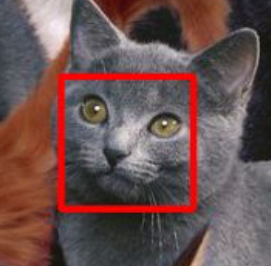
\includegraphics[width=3.3cm,height=3.3cm]{uTools_1651134324913.png}}
        \hspace{1cm}
        \subfloat[目标图像]{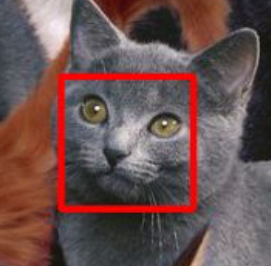
\includegraphics[width=2.4cm,height=1.5cm]{uTools_1651134324913.png}}
    \end{figure}
    图像宽高改变后,坐标点$(x,y)$和矩形框的宽高$(w,h)$按比例变化,源宽高为$(w_o,h_o)$,目标宽高为$(w_t,h_t)$:
    $$x'=\frac{xw_t}{w_o},y'=\frac{yh_t}{h_o}$$
\end{frame}

\begin{frame}
    \large
    @\textcolor{vscodeclass}{no\_grad}\textcolor{vscodebracket}{()}\\
    \vspace{0.2em}
    \textcolor{vscodedef}{def} \textcolor{vscodefuncation}{resizeBox}\textcolor{vscodebracket}{(}\\
    \vspace{0.2em}
    \qquad\textcolor{vscodeparameter}{orgsize}:\textcolor{vscodeclass}{Tuple}\textcolor{vscodecomment}{[}\textcolor{vscodeclass}{int},\textcolor{vscodeclass}{int}\textcolor{vscodecomment}{]},\\
    \vspace{0.2em}
    \qquad\textcolor{vscodeparameter}{tarsize}:\textcolor{vscodeclass}{Tuple}\textcolor{vscodecomment}{[}\textcolor{vscodeclass}{int},\textcolor{vscodeclass}{int}\textcolor{vscodecomment}{]},\\
    \vspace{0.2em}
    \qquad\textcolor{vscodeparameter}{boxes}:\textcolor{vscodeclass}{Tensor}\\
    \vspace{0.2em}
    \qquad\textcolor{vscodebracket}{)}->\textcolor{vscodeclass}{Tensor}:\\
    \vspace{0.2em}
    \qquad\textcolor{vscodeparameter}{orgsize},\textcolor{vscodeparameter}{tarsize}=\textcolor{vscodeclass}{Tensor}\textcolor{vscodebracket}{(}\textcolor{vscodeparameter}{orgsize}\textcolor{vscodebracket}{)},\textcolor{vscodeclass}{Tensor}\textcolor{vscodebracket}{(}\textcolor{vscodeparameter}{tarsize}\textcolor{vscodebracket}{)}\\
    \vspace{0.2em}
    \qquad\textcolor{vscodeparameter}{matrix}=\textcolor{vscodeclass}{torch}.\textcolor{vscodefuncation}{diag}\textcolor{vscodebracket}{(}\textcolor{vscodeparameter}{tarsize}/\textcolor{vscodeparameter}{orgsize}\textcolor{vscodebracket}{)}\\
    \vspace{0.2em}
    \qquad \textcolor{vscodereturn}{return} \textcolor{vscodeclass}{torch}.\textcolor{vscodefuncation}{cat}\textcolor{vscodebracket}{(}\textcolor{vscodecomment}{[}\textcolor{vscodeparameter}{boxes}\textcolor{vscode3bracket}{[}:,:\textcolor{vscodecomment}{2}\textcolor{vscode3bracket}{]}@\textcolor{vscodeparameter}{matrix},\textcolor{vscodeparameter}{boxes}\textcolor{vscode3bracket}{[}:,:\textcolor{vscodecomment}{2}\textcolor{vscode3bracket}{]}@\textcolor{vscodeparameter}{matrix}\textcolor{vscodecomment}{]},-\textcolor{vscodecomment}{1}\textcolor{vscodebracket}{)}
\end{frame}



\begin{frame}
    \vspace{0.5em}
    \noindent\large\textbf{非极大值抑制}\\
    \vspace{0.5em}
    非极大值抑制(NMS)主要用来去除重复的预测框,其输入是预测框数组与对应的置信度数组,算法过程如下:\\
    \vspace{0.5em}
    按置信的从大到小排序\\
    While 数组非空:\\
    \qquad 取出置信度最大的预测框 B\\
    \qquad B放入结果集\\
    \qquad 对于剩余数组当中每一个预测框b:\\
    \qquad \qquad if IoU(B,b)>阈值:\\
    \qquad \qquad \qquad 从数组中删除b\\

    \begin{figure}
        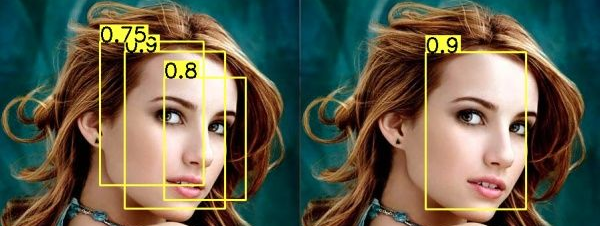
\includegraphics[width=0.7\linewidth]{NMS.png}
    \end{figure}

\end{frame}

\begin{frame}
    \large
    @\textcolor{vscodeclass}{no\_grad}\textcolor{vscodebracket}{()}\\
    \vspace{0.2em}
    \textcolor{vscodedef}{def}  \textcolor{vscodefuncation}{nms}\textcolor{vscodebracket}{(}\textcolor{vscodeparameter}{boxes}:\textcolor{vscodeclass}{Tensor},\textcolor{vscodeparameter}{score}:\textcolor{vscodeclass}{Tensor}, \textcolor{vscodeparameter}{threshold}:\textcolor{vscodeclass}{float}\textcolor{vscodebracket}{)}->\textcolor{vscodeclass}{Tensor}:\\
    \vspace{0.2em}
    \qquad\textcolor{vscodecomment}{\# boxes:(N,4) score:(N)}\\
    \vspace{0.2em}
    \qquad\textcolor{vscodeparameter}{\_},\textcolor{vscodeparameter}{indexes}=\textcolor{vscodeparameter}{score}.\textcolor{vscodefuncation}{sort}\textcolor{vscodebracket}{(}\textcolor{vscodeparameter}{descending}=\textcolor{vscodedef}{True}\textcolor{vscodebracket}{)}\\
    \vspace{0.2em}
    \qquad\textcolor{vscodeparameter}{result}=\textcolor{vscodebracket}{[]}\\
    \vspace{0.2em}
    \qquad\textcolor{vscodereturn}{while} \textcolor{vscodecomment}{0} \textcolor{vscodedef}{not in }\textcolor{vscodeparameter}{indexes}.\textcolor{vscodeparameter}{shape}:\\
    \vspace{0.2em}
    \qquad\qquad\textcolor{vscodeparameter}{result}.\textcolor{vscodefuncation}{append}\textcolor{vscodebracket}{(}\textcolor{vscodeparameter}{indexes}\textcolor{vscodecomment}{[0]}\textcolor{vscodebracket}{)}\\
    \vspace{0.2em}
    \qquad\qquad\textcolor{vscodeparameter}{temp\_boxes}=\textcolor{vscodeparameter}{boxes}\textcolor{vscodecomment}{[}\textcolor{vscodeparameter}{indexes}\textcolor{vscodecomment}{]}\\
    \vspace{0.2em}
    \qquad\qquad\textcolor{vscodeparameter}{ious}=\textcolor{vscodefuncation}{box\_iou}\textcolor{vscodebracket}{(}\textcolor{vscodeparameter}{temp\_boxes}\textcolor{vscodecomment}{[}:\textcolor{vscodecomment}{1]},\textcolor{vscodeparameter}{temp\_boxes}\textcolor{vscodecomment}{[1}:\textcolor{vscodecomment}{]}\textcolor{vscodebracket}{)[}\textcolor{vscodecomment}{0}\textcolor{vscodebracket}{]}\\
    \vspace{0.2em}
    \qquad\qquad\textcolor{vscodeparameter}{indexes}=\textcolor{vscodeparameter}{indexes}\textcolor{vscodebracket}{[}\textcolor{vscodecomment}{1}:\textcolor{vscodebracket}{][}\textcolor{vscodeparameter}{ious}<=\textcolor{vscodeparameter}{threshold}\textcolor{vscodebracket}{]}\\
    \vspace{0.2em}
    \qquad\textcolor{vscodereturn}{return} \textcolor{vscodeclass}{torch}.\textcolor{vscodefuncation}{stack}\textcolor{vscodebracket}{(}\textcolor{vscodeparameter}{result}\textcolor{vscodebracket}{)}
\end{frame}